\documentclass[12pt,t]{beamer}
% \documentclass[t]{beamer}
\usepackage[utf8]{inputenc}
\usepackage[catalan]{babel}
\usepackage{verbatim}
\usepackage{hyperref}
\usepackage{amsfonts,amssymb,amsmath,amsthm, wasysym}
\usepackage{listings}
\usepackage[T1]{fontenc}        
\usepackage{pgf}
\usepackage{epsdice}
\usepackage{pgfpages}
\usepackage{tikz}
%\usetikzlibrary{arrows,shapes,plotmarks,backgrounds,trees,positioning}
%\usetikzlibrary{decorations.pathmorphing,calc,snakes}
%\usepackage{marvosym}
%
\setbeamertemplate{footline}[frame number]
% \useoutertheme[footline=empty,subsection=true,compress]{infolines}
% \useoutertheme[footline=empty,subsection=true,compress]{miniframes}
% \usefonttheme{serif}

\setbeamertemplate{caption}[numbered]
\setbeamertemplate{navigation symbols}{}


\newcommand{\red}[1]{\textcolor{red}{#1}}
\newcommand{\green}[1]{\textcolor{green}{#1}}
\newcommand{\blue}[1]{\textcolor{blue}{#1}}
\newcommand{\gray}[1]{\textcolor{gray}{#1}}
\renewcommand{\emph}[1]{{\color{red}#1}}

\setbeamertemplate{frametitle}
{\begin{centering}
\medskip
\color{blue}
\textbf{\insertframetitle}
\medskip
\end{centering}
}
\usecolortheme{rose}
\usecolortheme{dolphin}
\mode<presentation>


\newcommand{\CC}{\mathbb{C}}
\newcommand{\RR}{\mathbb{R}}
\newcommand{\ZZ}{\mathbb{Z}}
\newcommand{\NN}{\mathbb{N}}
\newcommand{\KK}{\mathbb{K}}
\newcommand{\MM}{\mathcal{M}}
%\newcommand{\dbinom}{\displaystyle\binom}

\newcommand{\limn}{{\displaystyle \lim_{n\to\infty}}}
\renewcommand{\leq}{\leqslant}
\renewcommand{\geq}{\geqslant}
\def\tendeix{{\displaystyle\mathop{\longrightarrow}_{\scriptscriptstyle
n\to\infty}}}

\newcommand{\matriu}[1]{\left(\begin{matrix} #1 \end{matrix}\right)}

% \newcommand{\qed}{\hbox{}\nobreak\hfill\vrule width 1.4mm height 1.4mm depth 0mm
%     \par \goodbreak \smallskip}
%
% %
\theoremstyle{plain}
\newtheorem{teorema}{Teorema}
\newtheorem{prop}{Proposició}
\newtheorem{cor}{Coro\l.lari}
\theoremstyle{definition}
\newtheorem{exemple}{Exemple}
\newtheorem{defin}{Definició}
\newtheorem{obs}{Observació}

\newcounter{seccions}
\newcommand{\seccio}[1]{\addtocounter{seccions}{1}
\medskip\par\noindent\textbf{\theseccions.
#1}\smallskip\par }

\newcommand{\EM}{\Omega}
\newcommand{\PP}{\mathcal{P}}

\title[\red{Matemàtiques III}]{}
\author[]{}
\date{}



\begin{document}
\beamertemplatedotitem

\lstset{backgroundcolor=\color{green!50}}
\lstset{breaklines=true}
\lstset{basicstyle=\ttfamily}


\section{Intervals de confiança}

\begin{frame}
\vfill
\begin{center}
\gray{\LARGE Intervals de confiança}
\end{center}
\vfill
\end{frame}

\subsection{Definicions bàsiques}

\begin{frame}
\frametitle{El problema}
\vspace*{-1cm}

\begin{center}
\hspace*{-0.6cm}

\includegraphics[width=1.1\linewidth]{sanidade}
\end{center}
\vspace*{-1ex}

Amb un estimador, estimam el paràmetre amb una certa precisió, que depèn:
\medskip

\begin{itemize}
\item De la variabilitat de l'estimador
\medskip

\item De la mida de la mostra
\medskip

\item Del \emph{nivell de confiança} de l'estimació: com de segurs volem estar que l'estimació és correcta
\end{itemize}
\end{frame}


\begin{frame}
\frametitle{El problema}
\vspace*{-1cm}

\begin{center}
\hspace*{-0.5cm}

\includegraphics[width=1.1\linewidth]{plagiUIB1.jpg}\medskip

\hspace*{-0.4cm}

\includegraphics[width=1.05\linewidth]{plagiUIB3.jpg}\medskip

\hspace*{-0.5cm}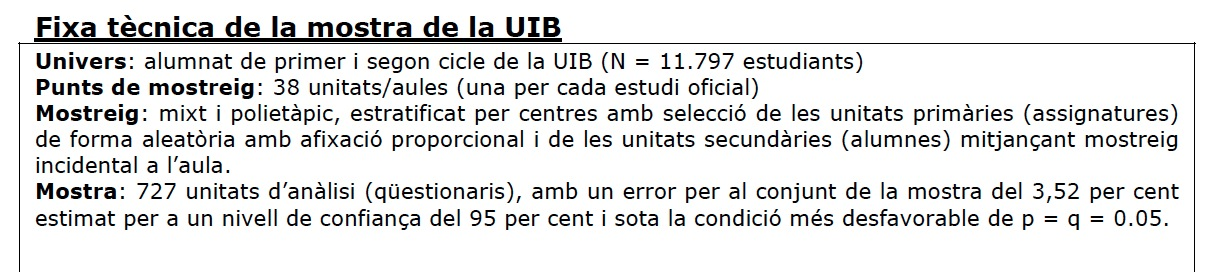
\includegraphics[width=1.1\linewidth]{plagiUIB2.jpg}
\end{center}
\vspace*{-1ex}

Per tant (per ara):
\begin{quote}
\red{Amb 95\% de confiança podem afirmar que entre un mínim d'un 73.1\% i un màxim d'un 80.1\% dels estudiants de la UIB
accepten\ldots}
\end{quote}
\end{frame}


\begin{frame}
\frametitle{El problema}
\vspace*{-0.5cm}

\begin{center}

\includegraphics[width=1\linewidth]{EPA3}
\end{center}
\end{frame}

\begin{frame}
\frametitle{Definicions bàsiques}

A l'\blue{Encuesta de Población Activa} (\blue{EPA}):

\begin{center}
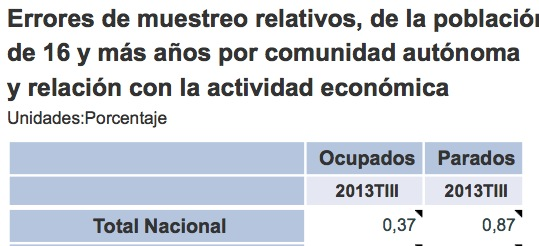
\includegraphics[width=0.6\linewidth]{EPA1}

{\scriptsize \url{http://www.ine.es/jaxi/tabla.do?per=03&type=db&divi=EPA&idtab=313}}
\medskip

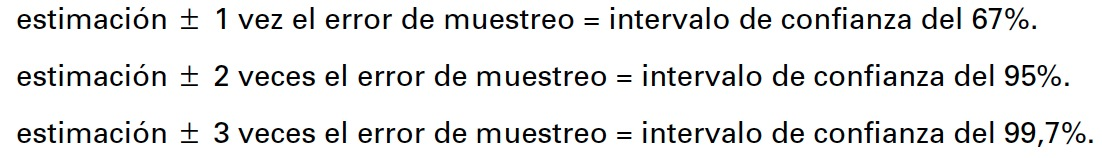
\includegraphics[width=\linewidth]{EPA2}


{\scriptsize \url{http://www.ine.es/docutrab/eval_epa/evaluacion_epa04.pdf}}
\end{center}
\end{frame}

\begin{frame}
\frametitle{El problema}
\vspace*{-2ex}

\blue{EPA d'octubre de 2013}: \smallskip
\begin{itemize}
\item El nombre estimat d'aturats a nivell nacional va ser de 5\,904\,700 \smallskip

\item L'error de mostreig va ser d'un 0.87\% \smallskip

\item Per tant, estam bastant segurs (nivell de confiança del 95\%) que el nombre d'aturats estava entre
$$
\begin{array}{rl}
\hspace*{-2ex} 5\,904\,700\!-\! 2\!\cdot \! 0.0087\!\cdot\! 5\,904\,700 & \hspace*{-1ex}=\! 5\,904\,700\!-\! 102\,742\\ &  \hspace*{-1ex}=\! 5\,801\,958\quad \mbox{ i}\\
\hspace*{-2ex} 5\,904\,700\!+\!2\!\cdot\! 0.0087\!\cdot\! 5\,904\,700 & \hspace*{-1ex}=\! 5\,904\,700\!+\! 102\,742\\ & \hspace*{-1ex}=\! 6\,007\,442
 \end{array}
 $$
 
 \item L'EPA de juny 2013 havia estimat el nombre d'aturats en 5\,977\,500
 \smallskip
 
 \item \red{No hi ha evidència que l'atur baixàs}
 \end{itemize}
\end{frame}







\begin{frame}
\frametitle{Definicions bàsiques}

Una \emph{estimació per intervals} d'un paràmetre poblacional és una regla per calcular, a partir d'una mostra, un interval on, amb una certa probabilitat (\emph{nivell de confiança}), es troba el  valor vertader del paràmetre
\bigskip


\end{frame}


\begin{frame}
\frametitle{Exemples}


\blue{Exemple:} 
Hem triat a l'atzar 50 estudiants de grau de la UIB, hem calculat les seves notes mitjanes de les assignatures del primer semestre, i la mitjana d'aquestes mitjanes ha estat un 6.3, amb una variància mostral  de 1.8\medskip

Determinau un interval que puguem afirmar amb probabilitat 95\% que conté la mitjana real de les notes mitjanes dels estudiants de grau de la UIB aquest primer semestre
\end{frame}


\begin{frame}
\frametitle{Exemples}


\blue{Exemple:} En un experiment s'ha mesurat el percentatge d'augment d'alcohol en sang a 40 persones després de prendre 4 canyes de cervesa. La mitjana i la desviació típica mostral d'aquests percentatges d'increment han estat
$$
\overline{x}=41.2,\quad \widetilde{s}=2.1
$$
Determinau un interval que puguem afirmar amb probabilitat 95\% que conté el percentatge d'augment mitjà d'alcohol en sang  (vertader) d'una persona després de beure quatre canyes de cervesa.


\end{frame}




\begin{frame}
\frametitle{Definicions bàsiques}

Donat un paràmetre $\theta$, l'interval $]A,B[$ és un \emph{interval de confiança} del
$(1-\alpha)\cdot 100\% $ per al paràmetre $\theta$ quan
$$
P(A<\theta<B)=1-\alpha
$$
El valor $(1-\alpha)\cdot 100\% $ (o també només el $1-\alpha$) rep el nom de \emph{nivell de confiança} 
\medskip

El valor $\alpha$ rep el nom de \emph{nivell de significació}
\medskip 


\blue{Exemple:} $]A,B[$ és un interval de confiança del $95\%$ (o de nivell de significació de 0.05) si
$$
P(A<\theta<B)=0.95
$$


\end{frame}




\begin{frame}
\frametitle{Definicions bàsiques}

\emph{Per defecte}, cercarem  intervals tals que la \emph{cua} de probabilitat sobrant $\alpha$ es reparteixi per igual a cada costat de l'interval:
$$
P(\theta<A)=P(\theta>B)=\frac{\alpha}{2}
$$
\begin{center}
\begin{tikzpicture}[thick,scale=0.8]%[>=stealth]%,yscale=0.5,xscale=0.7]
\draw (0,0)--(10,0);
\draw (3,0.3)--(3,-0.3);
\draw (7,0.3)--(7,-0.3);
\draw(3,-0.6) node {\small $A$}; 
\draw (7,-0.6) node {\small $B$}; 
\draw[red] (8.5,-0.3) node {\small $\alpha/2$}; 
\draw[red] (1.5,-0.3) node {\small $\alpha/2$}; 
\draw[red] (5,-0.3) node {\small $1-\alpha$}; 
\end{tikzpicture}
\end{center}


\blue{Exemple:} Per cercar  un interval de confiança  $]A,B[$ del $95\%$, cercarem $A,B$ de manera que 
$$
P(\theta<A)=0.025\quad\mbox{ i }\quad P(\theta>B)=0.025
$$


\end{frame}

\subsection{$\mu$ de població normal amb $\sigma$ coneguda}
\begin{frame}
\frametitle{Exemple: $\mu$ de població normal amb $\sigma$ coneguda}

Sigui $X$ una v.a. normal amb mitjana poblacional $\mu$ desconeguda i desviació típica poblacional $\sigma$ coneguda (a la pràctica, usualment, \emph{estimada en un experiment anterior})
\medskip

Sigui $X_1,\ldots,X_n$ una m.a.s. de $X$, amb mitjana mostral $\overline{X}$
\medskip

Volem determinar un interval de confiança per a $\mu$ amb un cert nivell de confiança (posem, 97.5\%):  un interval $]A,B[$ tal que
$$
P(A<\mu<B)=0.975
$$


\end{frame}

\begin{frame}
\frametitle{Exemple: $\mu$ de població normal amb $\sigma$ coneguda}

Sota aquestes condicions, sabem que
$$
Z=\frac{\overline{X}-\mu}{\sigma/\sqrt{n}}
$$
segueix una distribució normal estàndard
\medskip

Comencem calculant un interval centrat en $0$ on  $Z$ hi
tingui probabilitat $0.975$:
$$
\begin{array}{l}
0.975\!=\! P(-\delta<Z<\delta)\!=\!F_{Z}(\delta)\!-\!F_{Z}(-\delta)\!=\!
2 F_{Z}(\delta)\!-\!1\\[2ex]
F_{Z}(\delta)=\dfrac{1.975}{2}=0.9875\Rightarrow
\delta=\texttt{qnorm(0.9875)}=2.24
\end{array}
$$
\end{frame}


\begin{frame}
\frametitle{Exemple: $\mu$ de població normal amb $\sigma$ coneguda}
Per tant
$$
P(-2.24<Z<2.24)=0.975
$$
Substituint $Z=\dfrac{\overline{X}-\mu}{\sigma/\sqrt{n}}$
$$
\begin{array}{c}
P\left(-2.24<\dfrac{\overline{X}-\mu}{\sigma/\sqrt{n}}
<2.24\right)=0.975\\[3ex]
P\left(\overline{X} -2.24 \dfrac{\sigma}{\sqrt{n}}< \mu< \overline{X}+
2.24\dfrac{\sigma}{\sqrt{n}}\right)=0.975
\end{array}
$$
\end{frame}
\begin{frame}
\frametitle{Exemple: $\mu$ de població normal amb $\sigma$ coneguda}
Per tant, la probabilitat que la $\mu$ de la $X$ es trobi dins l'interval
$$
\left]\overline{X} -2.24 \frac{\sigma}{\sqrt{n}},
\overline{X}+ 2.24\frac{\sigma}{\sqrt{n}}
\right[
$$
és $0.975$: és un interval de confiança del 97.5\%
\medskip

\red{A més:}
\begin{itemize}
\item Centrat en $\overline{X}$
\medskip

\item El 0.025 de probabilitat restant està repartit per igual als dos costats de l'interval
\end{itemize}
\end{frame}

\begin{frame}
\frametitle{Exemple: $\mu$ de població normal amb $\sigma$ coneguda}


\begin{itemize}
\item \blue{Com a estimador:} Un 97.5\% de les ocasions que prenguem una mostra de mida $n$ de $X$, el vertader valor de $\mu$ es trobarà dins d'aquest interval 
\medskip

\item \blue{Per a una mostra concreta:} La probabilitat que, si  una $\mu$ ha produït aquesta mostra, aleshores estigui dins aquest interval concret, és del 97.5\%
\medskip

\item \blue{Ho entendrem com a}:  ``La probabilitat que $\mu$ estigui dins aquest interval  és del 97.5\%''
\medskip

\item \blue{Però és mentira} (\emph{abús de llenguatge}): La $\mu$ concreta és un valor fix, per tant que pertanyi a aquest interval concret té probabilitat 1 (si hi pertany) i 0 (si no hi pertany) 
\end{itemize}


\end{frame}




\begin{frame}
\frametitle{I.C. per a $\mu$ de població normal amb $\sigma$ coneguda}
\vspace*{-3ex}

\begin{teorema}
Sigui $X\sim N(\mu,\sigma)$ amb $\mu$ desconeguda i $\sigma$ coneguda.
\medskip

Prenem una m.a.s. de $X$ de mida $n$, amb mitjana $\overline{X}$.
\medskip

Un interval de confiança del $(1-\alpha)\cdot 100\%$ per a $\mu$  és 
$$
\left]\overline{X} -z_{1-\frac{\alpha}{2}} \frac{\sigma}{\sqrt{n}}, \overline{X}+z_{1-\frac{\alpha}{2}}\frac{\sigma}{\sqrt{n}}
\right[
$$
on $z_{1-\frac{\alpha}{2}}$ és el $(1-\frac{\alpha}{2})$-quantil de la normal  estàndard $Z$ (és a dir, $z_{1-\frac{\alpha}{2}}=F_Z^{-1}(1-\frac{\alpha}{2})$, o $P(Z\leq z_{1-\frac{\alpha}{2}})=1-\frac{\alpha}{2}$)
\end{teorema}

%(Recordau que $F_Z^{-1}(\frac{\alpha}{2})=-F_Z^{-1}(1-\frac{\alpha}{2})$)

\end{frame}


\begin{frame}
\frametitle{I.C. per a $\mu$ de població normal amb $\sigma$ coneguda}

Si $X$ és normal amb $\sigma$ coneguda, un interval de confiança per a $\mu$ del $(1-\alpha)\cdot 100\%$ és 
$$
\red{\overline{X} \pm z_{1-\frac{\alpha}{2}} \frac{\sigma}{\sqrt{n}}}:=\left]\overline{X} -z_{1-\frac{\alpha}{2}} \frac{\sigma}{\sqrt{n}}, \overline{X}+z_{1-\frac{\alpha}{2}}\frac{\sigma}{\sqrt{n}}
\right[
$$
Observau que està centrat en $\overline{X}$
\begin{center}
\begin{tabular}{c|c|c}
\blue{Confiança $1-\alpha$} & \blue{Significació $\alpha$} & \blue{$z_{1-\frac{\alpha}{2}}$}\\
 \hline
0.900\ & 0.100 &1.64 \\   
0.950 & 0.050 & 1.96\\
0.975 & 0.025 & 2.24 \\
0.990 & 0.010 & 2.58
\end{tabular}
\end{center}


\end{frame}

\begin{frame}[fragile]
\frametitle{I.C. per a $\mu$ de població normal amb $\sigma$ coneguda}
\vspace*{-3ex}

\small
\begin{verbatim}
ICZ=function(x,sigma,alpha){
  c(mean(x)-qnorm(1-alpha/2)*sigma/sqrt(length(x)), 
  mean(x)+qnorm(1-alpha/2)*sigma/sqrt(length(x)))
}
set.seed(5)
mu=1.5; sigma=1; alpha=0.05
Poblacio=rnorm(10^6,mu,sigma)
M=replicate(100,ICZ(sample(Poblacio,50,replace=T),
 sigma,alpha))
plot(1:10,type="n",xlim=c(1.2,1.8),ylim=c(0,100),
xlab="Valors",ylab="Replicacions")
seg.int=function(i){color="grey";
  if((mu<M[1,i]) | (mu>M[2,i])){color = "red"}
  segments(M[1,i],i,M[2,i],i,col=color,lwd=3)}
invisible(sapply(1:100,FUN=seg.int))
abline(v=mu,lwd=3)
\end{verbatim}
\end{frame}

\begin{frame}
\frametitle{I.C. per a $\mu$ de població normal amb $\sigma$ coneguda}

\begin{center}
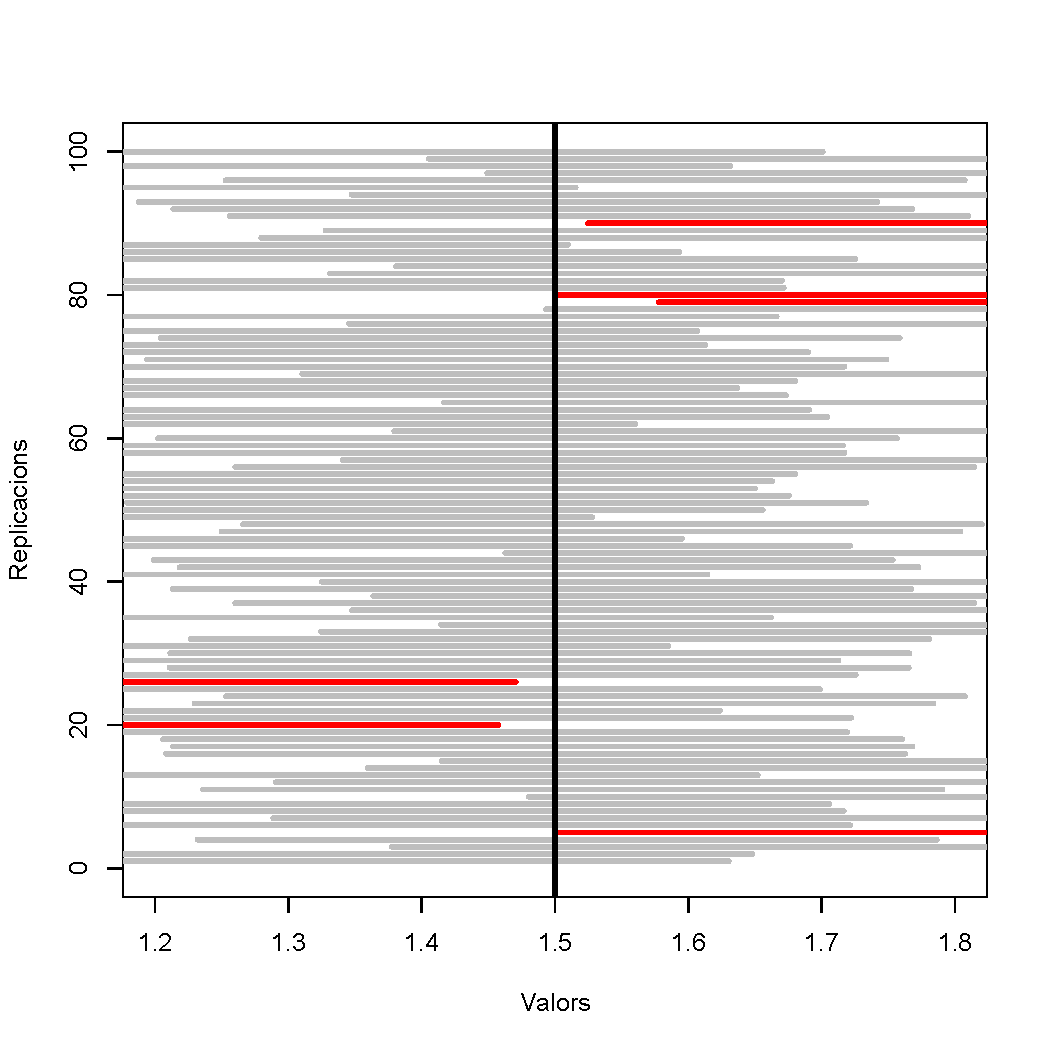
\includegraphics[width=0.5\linewidth]{intervals1}
\end{center}

\begin{block}{Alerta!}
De mitjana, un $\alpha100\%$ de les vegades, un interval de confiança del $(1-\alpha)100\%$  no contindrà el valor real del paràmetre
\end{block}

\end{frame}




\begin{frame}
\frametitle{Exemple}
\red{$\displaystyle
\left]\overline{X} -z_{1-\frac{\alpha}{2}} \frac{\sigma}{\sqrt{n}}, \overline{X}+z_{1-\frac{\alpha}{2}}\frac{\sigma}{\sqrt{n}}
\right[$}
\medskip


Prenem una m.a.s. de mida $n=16$ d'una v.a. normal amb $\sigma=4$ i $\mu$ desconeguda. La mitjana de la m.a.s. és 
$\overline{x}=20$.
\medskip

\blue{Calculau un interval de confiança del 97.5\% per a $\mu$}

\end{frame}



\begin{frame}
\frametitle{Exemple}
Tenim un aparell per mesurar volums de líquid. Per saber si està ben
calibrat, prenem 10 mostres consistents a emplenar un recipient d'un litre exacte i mesurar el seu contingut amb el nostre aparell. Obtenim els resultats de la taula següent:
\begin{center}
\begin{tabular}{c|c}
\hline
Volum mesurat  (en litres) & Freq. Absoluta\\
\hline
1.000 & 1 \\
1.002 & 2 \\
1.004 & 1 \\
1.006 & 2 \\
1.008 & 1 \\
1.010 & 2 \\
1.012 & 1 \\
\end{tabular}
\medskip

$\overline{x}=1.006$
\end{center}

\end{frame}

\begin{frame}[fragile]
\frametitle{Exemple}
\vspace*{-3ex}

\blue{Suposem que les mesures amb el nostre aparell del contingut d'aquest recipient 
segueixen una distribució normal amb variància poblacional coneguda $\sigma^2=0.01$. Calculau un interval de
confiança del 90\% per al resultat mitjà de mesurar un litre exacte amb el nostre aparell.}

\end{frame}


\begin{frame}
\frametitle{Amplada}

L'\emph{amplada} $A$ de l'interval de confiança 
$$
\left]\overline{X} -z_{1-\frac{\alpha}{2}} \frac{\sigma}{\sqrt{n}}, \overline{X}+z_{1-\frac{\alpha}{2}}\frac{\sigma}{\sqrt{n}}
\right[
$$
és
$$
\begin{array}{rl}
\red{A}& \displaystyle =\overline{X}+ z_{1-\frac{\alpha}{2}}\frac{\sigma}{\sqrt{n}}-\Big(\overline{X} -z_{1-\frac{\alpha}{2}}\frac{\sigma}{\sqrt{n}}\Big)\\[2ex] & \displaystyle =\red{2z_{1-\frac{\alpha}{2}}\frac{\sigma}{\sqrt{n}}}
\end{array}
$$

L'\emph{error màxim}, al nivell de confiança $(1-\alpha)$, que cometem en estimar $\mu$
per mitjà de $\overline{X}$ és la meitat d'aquesta amplada, 
$$
\red{z_{1-\frac{\alpha}{2}}\frac{\sigma}{\sqrt{n}}}
$$
\end{frame}

\begin{frame}
\frametitle{Amplada}

L'\emph{amplada} $A$ de l'interval de confiança 
$$
\left]\overline{X} -z_{1-\frac{\alpha}{2}} \frac{\sigma}{\sqrt{n}}, \overline{X}+z_{1-\frac{\alpha}{2}}\frac{\sigma}{\sqrt{n}}
\right[
$$
és
$$
A= 2z_{1-\frac{\alpha}{2}}\frac{\sigma}{\sqrt{n}}
$$

\blue{Observacions}
\begin{itemize}
\item Per a $n$ i $\alpha$ fixos, si $\sigma$ creix,
 $A$ creix
\smallskip

\item Per a $\sigma$ i $\alpha$ fixos, si $n$
creix,  $A$ decreix
\smallskip

\item Per a $\sigma$ i $n$ fixos, si
$1-\alpha$ creix, $A$ creix
\end{itemize}
\end{frame}




\begin{frame}
\frametitle{Amplada}

Si volem calcular la mida $n$ de la mostra per assegurar-nos que l'interval
de confiança per $\mu$ al nivell $(1-\alpha)$ té amplada prefixada màxima $A_0$ (o un
error màxim $A_0/2$), podem aïllar la $n$:
$$
A_0\geq 2z_{1-\frac{\alpha}{2}}\frac{\sigma}{\sqrt{n}}\Rightarrow
n\geq \left( 2 z_{1-\frac{\alpha}{2}}\frac{\sigma}{A_0}
\right)^2
$$
Donada $A_0$, prendrem
$$
\red{n=\left\lceil \left( 2 z_{1-\frac{\alpha}{2}}\frac{\sigma}{A_0}
\right)^2\right\rceil}
$$

\end{frame}


\begin{frame}
\frametitle{Exemple}

Recordau que les mesures amb el nostre aparell del contingut del recipient  d'1 litre exacte
segueixen una distribució normal amb variància poblacional coneguda $\sigma^2=0.01$
\medskip

\blue{Quantes mesures hauríem d'efectuar per obtenir la mesura mitjana amb un error màxim de 0.05 al nivell de confiança del 90\%?}




\end{frame}



\subsection{$\mu$ de població normal amb $\sigma$ desconeguda}

\begin{frame}
\frametitle{Distribució $t$ de Student}


Sigui $X\sim N(\mu,\sigma)$
\medskip

Sigui $X_1,\ldots,X_n$ una m.a.s. de $X$, amb mitjana $\overline{X}$ i desviació típica mostral $\widetilde{S}_{X}$
\medskip

\begin{teorema}
En aquestes condicions, la v.a.
$$
t=\frac{\overline{X}-\mu}{\widetilde{S}_{X}/\sqrt{n}}
$$
segueix una distribució \emph{$t$ de Student} amb $n-1$ graus de llibertat, \red{$t_{n-1}$}
\end{teorema}
\medskip

\red{$\widetilde{S}_{X}/\sqrt{n}$}: l'\emph{error mostral}, estima l'error estàndard $\sigma/\sqrt{n}$


\end{frame}



\begin{frame}
\frametitle{Distribució $t$ de Student}


La distribució $t$ de Student amb $\nu$ graus de llibertat, \red{$t_{\nu}$}:
\medskip

\begin{itemize}
\item  Té densitat
$$
f_{t_\nu}(x) = \frac{\Gamma(\frac{\nu+1}{2})} {\sqrt{\nu\pi}\,\Gamma(\frac{\nu}{2})} \Big(1+\frac{x^2}{\nu} \Big)^{-\frac{\nu+1}{2}}
$$
on $\Gamma(x)=\int_{0}^{\infty} t^{x-1}e^{-t}\, dt$ si $x> 0$. 
\bigskip

\item La distribució està tabulada (\emph{Teniu les taules a Campus Extens}), i amb R és \texttt{t}

\end{itemize}

\end{frame}




\begin{frame}
\frametitle{Distribució $t$ de Student}

Sigui $t_{\nu}$ una v.a. que segueix la distribució $t$ de
Student amb $\nu$ graus de llibertat
\medskip

\begin{itemize}
\item $E(t_{\nu})=0$  si $\nu>1$ i $Var(t_{\nu})=\dfrac{\nu}{\nu-2}$ si $\nu>2$
\medskip

\item La seva funció de distribució és simètrica respecte de $E(t_{\nu})=0$ (com la d'una $N(0,1)$):
$$
P(t_{\nu}\leq -x)=P(t_{\nu}\geq x)=1-P(t_{\nu}\leq x)
$$

\item Si $\nu$ és gran, la seva distribució és aproximadament la de $N(0,1)$ (però amb més variància: un poc més aplatada)
\end{itemize}

\end{frame}

\begin{frame}
\frametitle{Distribució $t$ de Student}
\vspace*{-1cm}

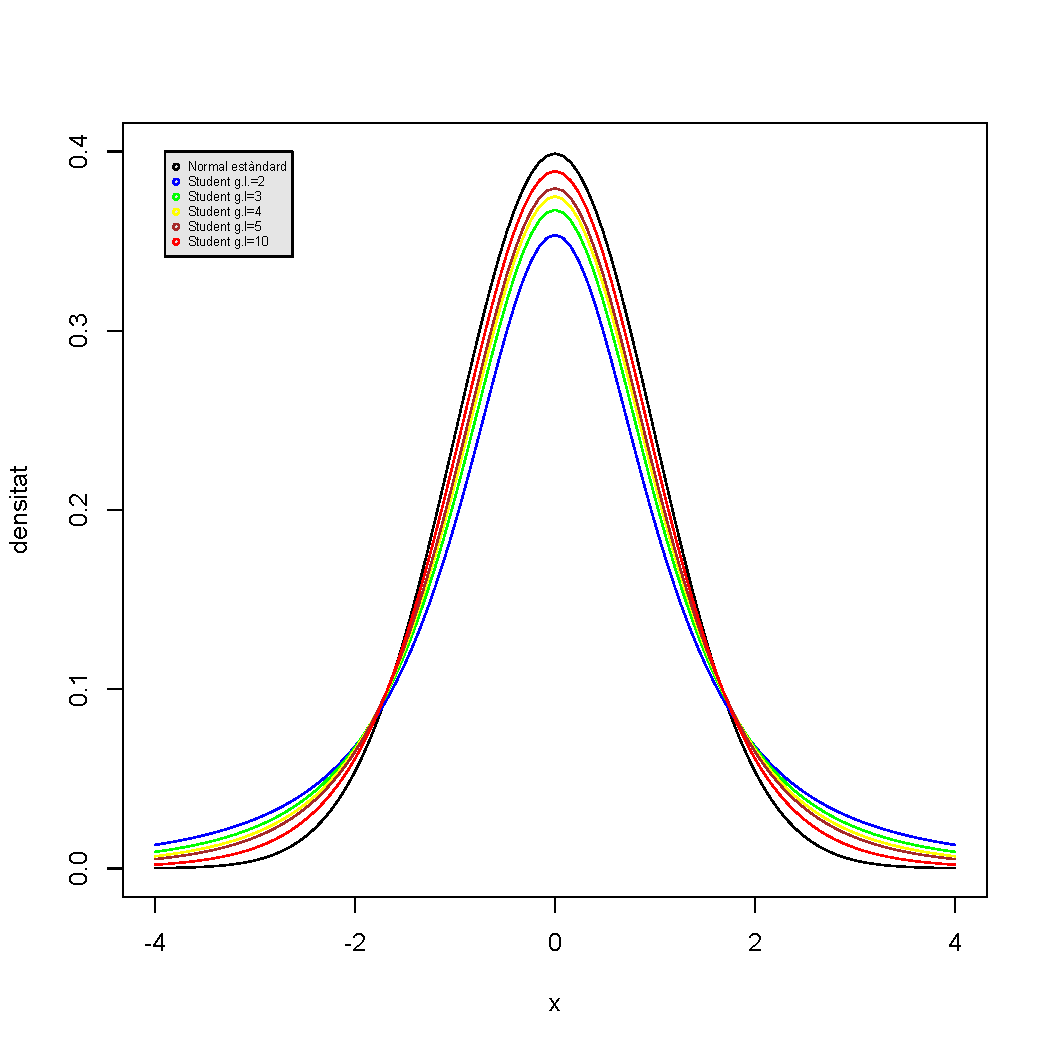
\includegraphics[width=0.95\linewidth]{tstud-div.pdf}
\end{frame}


\begin{frame}
\frametitle{Distribució $t$ de Student}

Indicarem amb
\red{$t_{\nu,q}$} el  $q$-quantil d'una  v.a.  $X_{t_{\nu}}$ que segueix una distribució   $t_\nu$:
$$
P(X_{t_{\nu}}\leq t_{\nu,q})=q
$$
Per simetria,
\red{$t_{\nu,q}=-t_{\nu,1-q}$}
\vspace*{-1ex}

\begin{center}
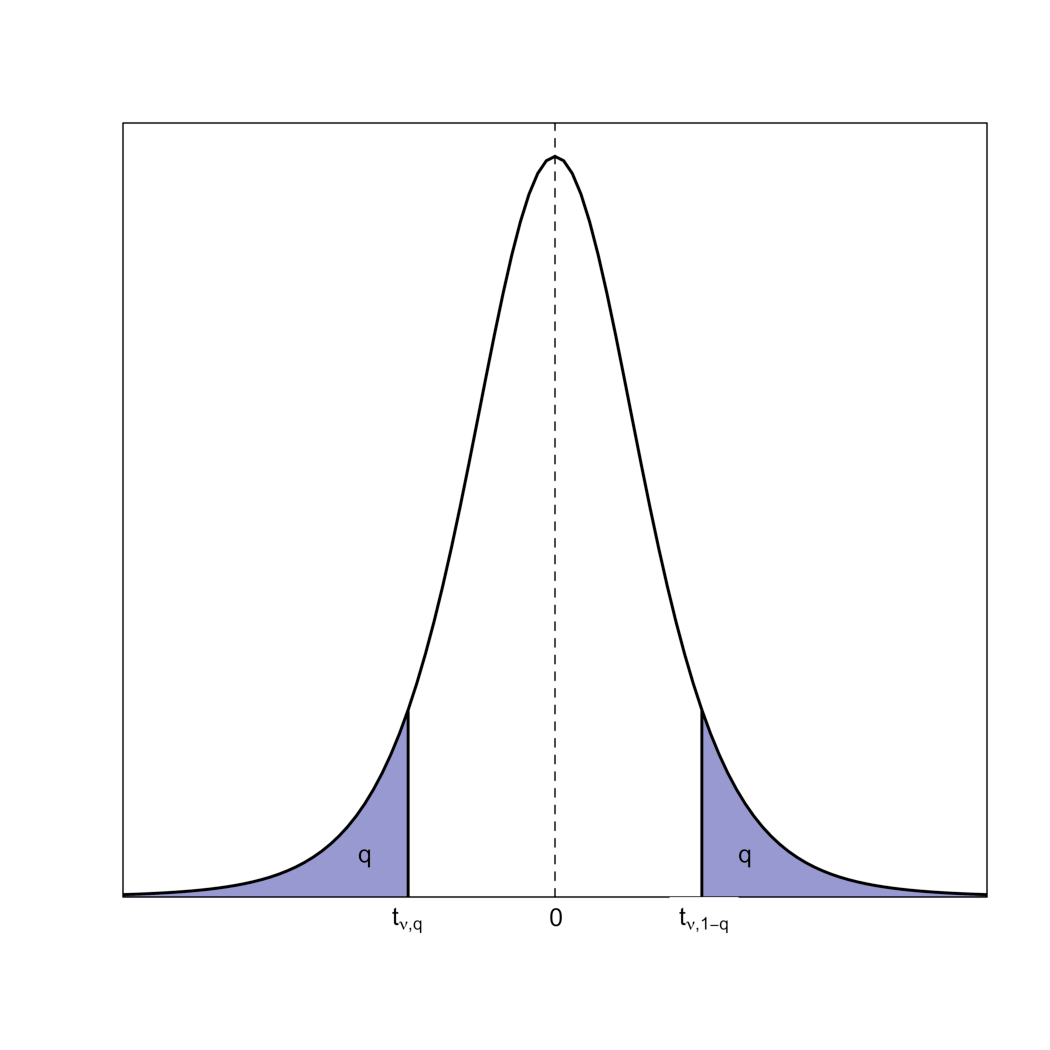
\includegraphics[width=0.6\linewidth]{quantilt}
\end{center}
\end{frame}


\begin{frame}
\frametitle{$\mu$ de població normal amb $\sigma$ desconeguda}

Considerem  la situació següent:
\begin{itemize}
\item  $X$ una v.a.  normal amb $\mu$ i $\sigma$ desconegudes

\item $X_1,\ldots,X_n$ una m.a.s. de $X$  de mida $n$, amb mitjana $\overline{X}$ i variància mostral $\widetilde{S}_X^2$
\end{itemize}


\begin{teorema}
En aquestes condicions, un interval  de confiança del $(1-\alpha)\cdot 100\%$ per a $\mu$
és  
$$
\left] 
\overline{X}-t_{n-1,1-\frac{\alpha}{2}} \frac{\widetilde{S}_{X}}{\sqrt{n}},
\overline{X}+t_{n-1,1-\frac{\alpha}{2}}\frac{\widetilde{S}_{X}}{\sqrt{n}} \right[
$$
\end{teorema}

\end{frame}

%
%
%\begin{frame}[fragile]
%\frametitle{$\mu$ de població normal amb $\sigma$ desconeguda}
%\vspace*{-5ex}
%
%\small
%\begin{verbatim}
%ICT=function(x,alpha){
%c(mean(x)-qt(1-alpha/2,length(x)-1)
%  *sd(x)/sqrt(length(x)),
%mean(x)+qt(1-alpha/2,length(x)-1)
%  *sd(x)/sqrt(length(x)))}
%set.seed(5)
%mu=1.5; sigma=0.4; alpha=0.05
%Poblacio=rnorm(10^6,mu,sigma)
%M=replicate(100,ICT(sample(Poblacio,15,replace=T),
%  alpha))
%plot(1:10,type="n",xlim=c(1.2,1.8),ylim=c(0,100),
%xlab="Valors",ylab="Replicacions")
%for(i in 1:100){color="grey";
%if((mu<M[1,i]) | (mu > M[2,i])){color = "red"}
%segments(M[1,i],i,M[2,i],i,col=color,lwd=3)}
%abline(v=mu,lwd=3)
%\end{verbatim}
%\end{frame}
%
%\begin{frame}
%\frametitle{$\mu$ de població normal amb $\sigma$ desconeguda}
%
%\begin{center}
%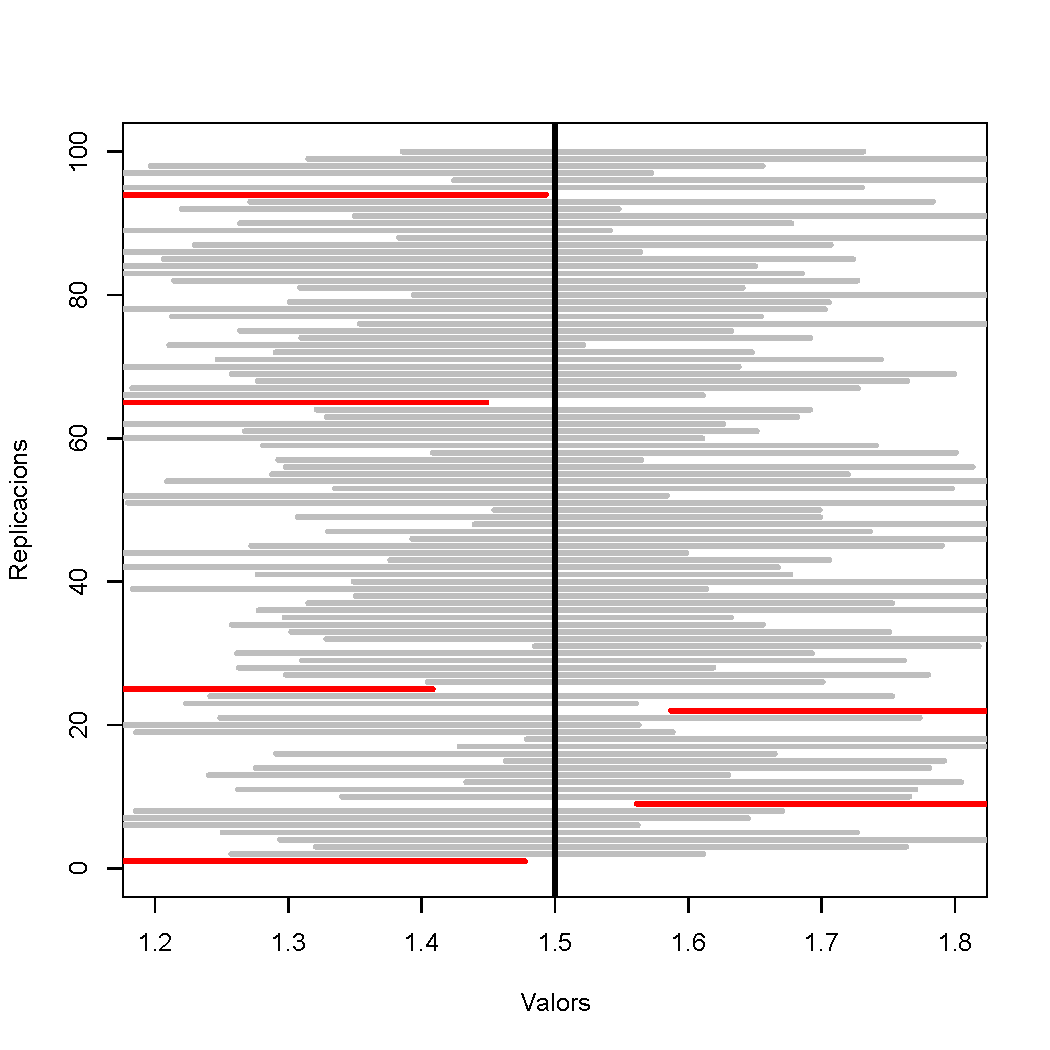
\includegraphics[width=0.7\linewidth]{intervals2}
%\end{center}
%\end{frame}
%
%
%
%
%



\begin{frame}
\frametitle{Exemple}

L'empresa \textsl{RX-print} ofereix una impressora de radiografies d'altíssima qualitat. En la seva publicitat afirma que els seus
cartutxos imprimeixen una mitjana de 500 radiografies amb l'especificació: 
\medskip

\blue{\texttt{Dades tècniques: Mostra mensual de mida $n=25$,
població suposada normal, nivell de confiança del 90\%}}
\medskip 

Uns radiòlegs desitgen comprovar aquestes afirmacions i prenen una
mostra a l'atzar de mida $n=25$, obtenint
una mitjana de $\overline{x}=518$ radiografies i una desviació típica mostral
$\widetilde{s}=40$
\medskip

Amb aquesta mostra, la mitjana poblacional anunciada pel fabricant cau dins de l'interval de confiança del 90\%?
\end{frame}

\begin{frame}[fragile]
\frametitle{Exemple}
Cal calcular l'interval de confiança per a $\mu$ amb 
$$
n=25, \overline{x}=518, \widetilde{s}=40, \alpha=0.1
$$
Serà
$$
\left] 
\overline{x}-t_{24,0.95} \frac{\widetilde{s}}{\sqrt{n}},
\overline{x}+t_{24,0.95} \frac{\widetilde{s}}{\sqrt{n}}\right[
$$
Mirant en les taules de la t de Student, obtenim $t_{24,0.95}=1.71$
\begin{verbatim}
> qt(0.95,24)
[1] 1.710882
\end{verbatim}

Operant: $]504.32,531.68[$, i no conté el 500 (però s'equivoca a favor del consumidor!)
\end{frame}

\begin{frame}
\frametitle{Observacions}

\begin{itemize}
\item L'interval de confiança obtingut està centrat en $\overline{X}$
\medskip

\item La fórmula
$$
\left] 
\overline{X}-t_{n-1,1-\frac{\alpha}{2}} \frac{\widetilde{S}_{X}}{\sqrt{n}},
\overline{X}+t_{n-1,1-\frac{\alpha}{2}}\frac{\widetilde{S}_{X}}{\sqrt{n}} \right[
$$
per a l'interval de confiança del $(1-\alpha)\cdot 100\%$ es pot fer servir quan $X$ és normal i $n$ qualsevol
\bigskip


\item Si $n$ és gran $t_{n-1,1-\frac{\alpha}{2}}\approx z_{1-\frac{\alpha}{2}}$ i podem \emph{aproximar-lo} amb
$$
\left] 
\overline{X}-z_{1-\frac{\alpha}{2}} \frac{\widetilde{S}_{X}}{\sqrt{n}},
\overline{X}+z_{1-\frac{\alpha}{2}}\frac{\widetilde{S}_{X}}{\sqrt{n}} \right[
$$
\end{itemize}


\end{frame}







\subsection{$\mu$ per a mostres grans}

\begin{frame}
\frametitle{$\mu$ per a mostres grans}

Considerem ara la situació següent:
\begin{itemize}
\item  $X$ una v.a.  \emph{qualsevol} amb mitjana poblacional $\mu$ desconeguda i desv. típ. $\sigma$ coneguda

\item $X_1,\ldots,X_n$ una m.a.s. de $X$, amb mitjana $\overline{X}$

\item \emph{$n$ és gran} (posem, $n\geq 40$)
\end{itemize}

\begin{teorema}
En aquestes condicions, podem prendre com a interval  de confiança del $(1-\alpha)\cdot 100\%$ per a $\mu$
$$
\left]\overline{X}-z_{1-\frac{\alpha}{2}}\frac{\sigma}{\sqrt{n}},
    \overline{X}+z_{1-\frac{\alpha}{2}}\frac{\sigma}{\sqrt{n}}\right[
$$
\end{teorema}



\end{frame}


\begin{frame}
\frametitle{$\mu$ per a mostres grans}

Considerem ara la situació següent:
\begin{itemize}
\item  $X$ una v.a.  \emph{qualsevol} amb mitjana poblacional $\mu$ desconeguda  \emph{i desv. típ. $\sigma$ desconeguda}

\item $X_1,\ldots,X_n$ una m.a.s. de $X$, amb mitjana $\overline{X}$ \emph{i desviació típica mostral $\widetilde{S}_X$}

\item \emph{$n$ és gran} (posem, $n\geq 40$)
\end{itemize}


\begin{block}{``Teorema''}
En aquestes condicions, es recomana prendre com a interval  de confiança del $(1-\alpha)\cdot 100\%$ per a $\mu$
$$
\left]\overline{X}-z_{1-\frac{\alpha}{2}}\frac{\widetilde{S}_X}{\sqrt{n}},
    \overline{X}+z_{1-\frac{\alpha}{2}}\frac{\widetilde{S}_X}{\sqrt{n}}\right[
$$
\end{block}



\end{frame}

%
%\begin{frame}[fragile]
%\frametitle{$\mu$ per a mostres grans}
%\vspace*{-2ex}
%
%\small
%\begin{verbatim}
%ICZ2=function(x,alpha){
%  c(mean(x)-qnorm(1-alpha/2)*sd(x)/sqrt(length(x)), 
%  mean(x)+qnorm(1-alpha/2)*sd(x)/sqrt(length(x)))
%}
%set.seed(15)
%lambda=1.5; alpha=0.05
%Poblacio=rpois(10^6,lambda)
%M=replicate(100,ICZ(sample(Poblacio,40,replace=T),
%  alpha))
%plot(1:10,lwd=3,xlim=c(1.2,1.8),ylim=c(0,100),
%xlab="Valors",ylab="Replicacions")
%for(i in 1:100){
%  color="grey";
%  if((mu<M[1,i]) | (mu > M[2,i])){color = "red"}
%  segments(M[1,i],i,M[2,i],i,col=color,lwd=3)
%}
%abline(v=mu,lwd=3)
%\end{verbatim}
%\end{frame}
%
%\begin{frame}
%\frametitle{$\mu$ per a mostres grans}
%
%\begin{center}
%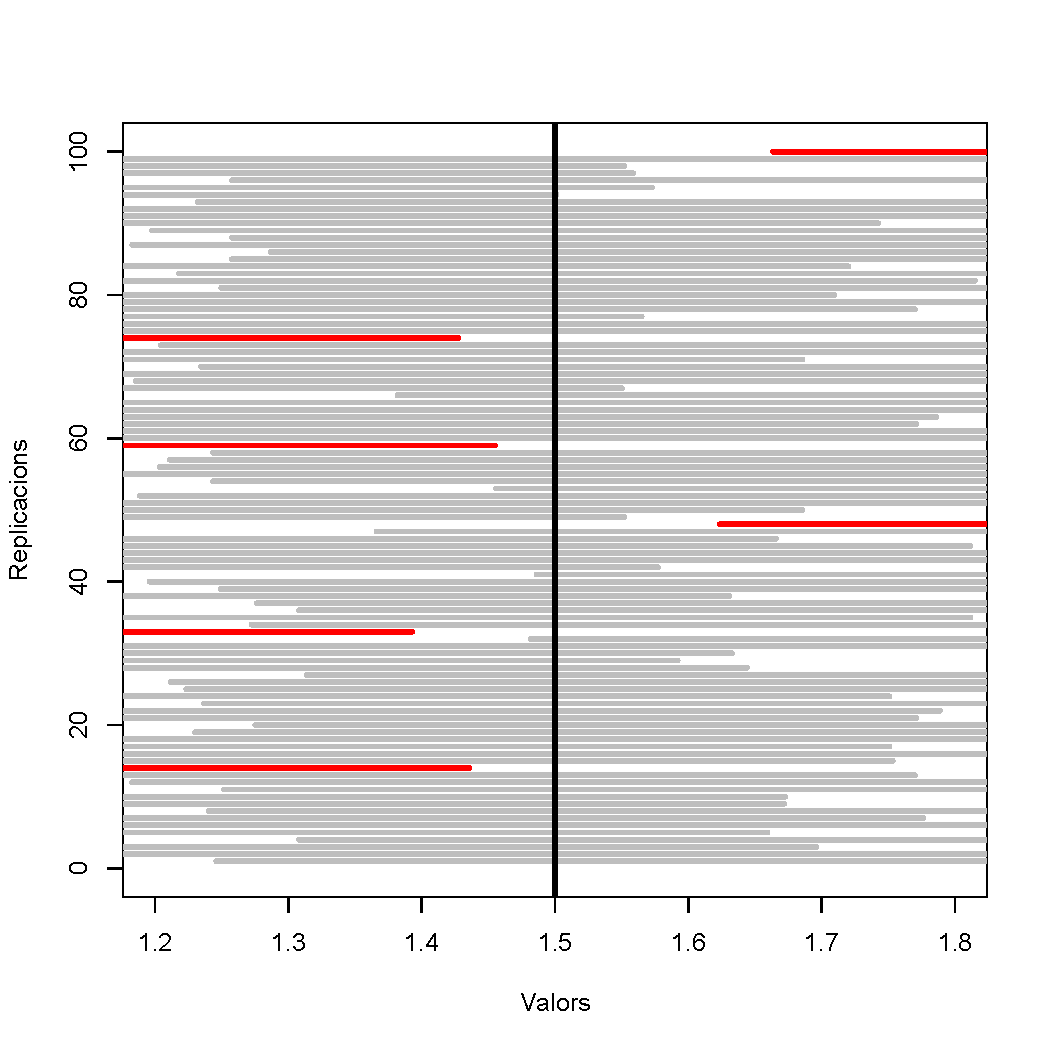
\includegraphics[width=0.7\linewidth]{intervals3}
%\end{center}
%\end{frame}
%
%




\begin{frame}
\frametitle{Exemple}
\vspace*{-2ex}

En un experiment s'ha mesurat el percentatge d'augment d'alcohol en sang a 40 persones després de prendre 4 canyes de cervesa. La mitjana i la desviació típica mostral d'aquests percentatges d'increment han estat
$$
\overline{x}=41.2,\quad \widetilde{s}=2.1
$$
Determinau un interval que puguem afirmar amb probabilitat 95\% que conté el  percentatge d'augment mitjà d'alcohol en sang d'una persona després de beure quatre canyes de cervesa.
\medskip


Ens demanen un \emph{interval de confiança del 95\%} per a $\mu$ de la v.a. $X$ ``percentatge d'augment d'alcohol en sang d'una persona després de beure quatre canyes de cervesa''


\end{frame}


\begin{frame}
\frametitle{Exemple}

No sabem com és $X$, però $n=40$ és gran
\medskip

Podem emprar
$$
\left]\overline{x}-z_{1-\frac{\alpha}{2}}\frac{\widetilde{s}}{\sqrt{n}},
    \overline{x}+z_{1-\frac{\alpha}{2}}\frac{\widetilde{s}}{\sqrt{n}}\right[
$$
on
$$
\begin{array}{c}
n=40,\overline{x}=41.2,\widetilde{s}=2.1,\\[1ex]
\alpha=0.05\Rightarrow z_{1-\frac{\alpha}{2}}=z_{0.975}=1.96
\end{array}
$$

$$
]40.55, 41.85[
$$
\medskip

Podem afirmar amb un 95\% de confiança que l'augment mitjà d'alcohol en sang d'una persona després de beure quatre canyes de cervesa està entre el $40.55\%$ i el $41.85\%$


\end{frame}



\begin{frame}
\frametitle{Exemple}
\vspace*{-2ex}

S'ha pres una mostra de sang a 1000 adults sans i s'hi ha mesurat la quantitat  de calci (en mg per dl de sang). S'ha obtingut una mitjana mostral de 9.5 mg/dl amb una desviació típica mostral de 0.5 mg/dl. 
\medskip

\blue{Trobau un interval de confiança del 95\% per a la quantitat mitjana de calci en sang en un adult sa}

\end{frame}



\begin{frame}
\frametitle{Amplada}

L'amplada de 
$$
\left]\overline{X}-z_{1-\frac{\alpha}{2}}\frac{\widetilde{S}_X}{\sqrt{n}},
    \overline{X}+z_{1-\frac{\alpha}{2}}\frac{\widetilde{S}_X}{\sqrt{n}}\right[
$$
és 
$$
A=2z_{1-\frac{\alpha}{2}}\frac{\widetilde{S}_X}{\sqrt{n}}
$$
Per determinar $n$ (gran) que doni com a màxim una amplada $A$ prefixada, ens cal $\widetilde{S}_X$, que depèn de la mostra.
\medskip

 Solucions:
\begin{itemize}
\item Si sabem la desv. típ. poblacional $\sigma$, l'empram per aproximar $\widetilde{S}_X$

\item Si hem pres una mostra prèvia (\emph{pilot}), n'empram la desviació típica mostral per estimar $\sigma$

\end{itemize}



\end{frame}



\begin{frame}
\frametitle{Amplada}

\begin{block}{}
D'una població $X$ n'hem pres una  \emph{m.a.s.\ pilot} que ha tingut una desviació típica mostral $\widetilde{s}_{pilot}$.
\medskip

Estimarem que la mida mínima $n$ d'una m.a.s.\ de $X$ que doni un interval de confiança per a $\mu_X$ de nivell de confiança $1-\alpha$ i amplada màxima $A_0$ és
$$
n=\left\lceil \Big(2z_{1-\frac{\alpha}{2}}\frac{\widetilde{s}_{pilot}}{A_0}\Big)^2\right\rceil
$$
\end{block}



\end{frame}





\begin{frame}
\frametitle{Exemple}

Volem estimar l'alçada mitjana dels estudiants de la UIB. Cercam  un interval de confiança del 99\% amb una precisió màxima de 1 cm. En una mostra pilot de 25 estudiants, obtinguérem 
$$
\overline{x} = 170\mbox{ cm}, \widetilde{s}=10\mbox{ cm}
$$
Basant-nos en aquestes dades, quina mida hauria de tenir la mostra per assolir el nostre objectiu?

\end{frame}

\subsection{$p$ per a mostres petites}

\begin{frame}
\frametitle{$p$ per a mostres petites}

Considerem la situació següent:
\begin{itemize}
\item  $X$ una v.a. Bernoulli amb $p$ desconeguda

\item $X_1,\ldots,X_n$ una m.a.s. de $X$, amb nombre d'èxits $x$ i per tant freqüència relativa d'èxits $\widehat{p}_{X}=x/n$
\end{itemize}

Recordau que $x$ és $B(n,p)$

\begin{block}{Mètode ``exacte'' de Clopper-Pearson}
Un interval de confiança $]p_0,p_1[$ del $(1-\alpha)100\%$ per a $p$ s'obté trobant el $p_0$ més gran i el $p_1$ més petit tals que
$$
\displaystyle\sum_{k=x}^np_0^k(1-p_0)^{n-k}\leq \frac{\alpha}{2},\qquad
\displaystyle\sum_{k=0}^xp_1^k(1-p_1)^{n-k}\leq \frac{\alpha}{2}
$$
\end{block}
A mà (consultant taules) és una feinada.

\end{frame}




\begin{frame}[fragile]
\frametitle{$p$ per a mostres petites}
\vspace*{-2ex}

El paquet \texttt{epitools} porta
\begin{center}
{\tt binom.exact(èxits,mida,conf.)}
\end{center}
per calcular-ho.
\medskip

\blue{De 10 pacients tractats amb un medicament, 2 s'han curat. Donau un interval de confiança del 95\% per a la proporció $p$ de pacients que aquest medicament cura.}
\begin{verbatim}
> install.packages("epitools",dep=TRUE)
> library(epitools)
> round(binom.exact(2,10,0.95),3)
  x  n proportion lower upper conf.level
1 2 10        0.2 0.025 0.556       0.95
\end{verbatim}
Dóna $]0.025,0.556[$
\end{frame}






\subsection{$p$ per a mostres grans}


\begin{frame}
\frametitle{$p$ per a mostres grans I}

Considerem ara la situació següent:
\begin{itemize}
\item  $X$ una v.a. Bernoulli amb $p$ desconeguda

\item $X_1,\ldots,X_n$ una m.a.s. de $X$, amb $n$  gran (per exemple, $n\geq 40$) i freqüència relativa d'èxits $\widehat{p}_{X}$
\end{itemize}
\medskip

En aquestes condicions (pel T.C.L.), 
$$
Z=\dfrac{\widehat{p}_{X}-p}
{\sqrt{\frac{p(1-p)}{n}}}\approx N(0,1)
$$
\end{frame}


\begin{frame}
\frametitle{$p$ per a mostres grans I}
Per tant
$$
P\left(-z_{1-\frac{\alpha}{2}}\leq \dfrac{\widehat{p}_{X}-p}
{\sqrt{\frac{p(1-p)}{n}}}\leq z_{1-\frac{\alpha}{2}}\right)=1-\alpha
$$
i aïllant la $p$ obtenim:
\end{frame}


\begin{frame}
\frametitle{$p$ per a mostres grans I}
\begin{block}{Mètode de Wilson}
En aquestes condicions, un interval  de confiança del $(1-\alpha)\cdot 100\%$ per a $p$
és  (posant $\widehat{q}_{X}=1-\widehat{p}_{X}$)
$$
\begin{array}{l}
\displaystyle \left]\frac{\widehat{p}_{X}+\frac{z_{1-{\alpha}/{2}}^2}{2n}-z_{1-{\alpha}/{2}}\sqrt{\frac{\widehat{p}_{X}\widehat{q}_{X}}{n}+\frac{z_{1-{\alpha}/{2}}^2}{4n^2}}}{1+\frac{z_{1-{\alpha}/{2}}^2}{n}}\right.,\\[2ex]
\hspace*{2cm} \displaystyle \left.\frac{\widehat{p}_{X}+\frac{z_{1-{\alpha}/{2}}^2}{2n}+z_{1-{\alpha}/{2}}\sqrt{\frac{\widehat{p}_{X}\widehat{q}_{X}}{n}+\frac{z_{1-{\alpha}/{2}}^2}{4n^2}}}{1+\frac{z_{1-{\alpha}/{2}}^2}{n}}\right[
\end{array}
$$
\end{block}
\medskip

\texttt{binom.wilson} del paquet \texttt{epitools}

\end{frame}



\begin{frame}
\frametitle{$p$ per a mostres grans II}

Considerem ara la situació següent:
\begin{itemize}
\item  $X$ una v.a. Bernoulli amb $p$ desconeguda

\item $X_1,\ldots,X_n$ una m.a.s. de $X$, amb $n$ més gran i $\widehat{p}_{X}$ enfora de 0 i 1. Per exemple, tal que:
$$
n\geq 100, n\widehat{p}_{X}\geq 10,  n(1-\widehat{p}_{X})\geq 10
$$
\end{itemize}
\medskip



\begin{block}{Fórmula de Laplace (1812)}
En aquestes condicions, es pot prendre com a interval  de confiança del $(1-\alpha)\cdot 100\%$ per a $p$
$$
\left]\widehat{p}_{X}-z_{1-\frac{\alpha}{2}}\sqrt{\frac{\widehat{p}_{X}
(1-\widehat{p}_{X})}{n}},
\widehat{p}_{X}+z_{1-\frac{\alpha}{2}}\sqrt{\frac{\widehat{p}_{X}
(1-\widehat{p}_{X})}{n}}\right[$$
\end{block}
\end{frame}



\begin{frame}
\frametitle{Exemple}

En una mostra aleatòria de 500 famílies amb nins en edat escolar es
va trobar que 340 introduïen fruita de forma diària en la dieta dels seus fills
\medskip

Cercau un interval de confiança del 95\% per a la proporció real de
famílies d'aquesta ciutat amb nins en edat escolar que incorporen fruita fresca de
forma diària en la dieta dels seus fills


\end{frame}
\begin{frame}
\frametitle{Exemple}

$X=$ ``Aportar diàriament fruita a la dieta dels fills''\\
 és $Be(p)$, i cercam interval de confiança del 95\% per a $p$
\bigskip

Com que $n=500\geq 100$, $n\widehat{p}_X=340\geq 10$ i $n(1-\widehat{p}_X)=160\geq 10$, podem emprar
$$
\left]\widehat{p}_{X}-z_{1-\frac{\alpha}{2}}\sqrt{\frac{\widehat{p}_{X}
(1-\widehat{p}_{X})}{n}},
\widehat{p}_{X}+z_{1-\frac{\alpha}{2}}\sqrt{\frac{\widehat{p}_{X}
(1-\widehat{p}_{X})}{n}}\right[
$$
amb
$$
\begin{array}{c}
n=500, \widehat{p}_{X}=\dfrac{340}{500}=0.68,\\[1ex]
 \alpha=0.05\Rightarrow z_{1-\frac{\alpha}{2}}=z_{0.975}=1.96
\end{array}
$$
Dóna 
$$
\red{]0.639,0.721[}
$$

\end{frame}

\begin{frame}[fragile]
\frametitle{Exemple}


Amb els altres mètodes:
\begin{verbatim}
> round(binom.exact(340,500,0.95),3)
    x   n proportion lower upper conf.level
1 340 500       0.68 0.637 0.721       0.95
> round(binom.wilson(340,500,0.95),3)
    x   n proportion lower upper conf.level
1 340 500       0.68 0.638 0.719       0.95
\end{verbatim}
Donen:
\medskip

\begin{itemize}
\item Clopper-Pearson: $]0.637,0.721[$
\medskip

\item Wilson: $]0.638, 0.719[$
\medskip

\item Laplace: $]0.639,0.721[$
\end{itemize}

\end{frame}

\begin{frame}
\frametitle{Exemple}

\blue{En un assaig d'un nou tractament de quimioteràpia, en una mostra de $n$ (gran) malalts tractats, cap desenvolupà càncer testicular com a efecte secundari. Trobau un interval de confiança al 95\% per a la proporció de malalts tractats amb aquesta quimio que desenvolupen càncer testicular.}
\vspace*{4cm}

\red{Els metges empren $\Big]0,\dfrac{3}{n}\Big[$ (la regla del 3)}


\end{frame}


\begin{frame}
\frametitle{Observacions}
\begin{itemize}
\item El mètode de Wilson dóna un I.C. centrat en
$$
\frac{\widehat{p}_{X}+\frac{z_{1-{\alpha}/{2}}^2}{2n}}{1+\frac{z_{1-{\alpha}/{2}}^2}{n}}
=\frac{2n\widehat{p}_{X}+ z_{1-\frac{\alpha}{2}}^2}{2n+2 z_{1-\frac{\alpha}{2}}^2}
$$

\item No es coneix una fórmula per al centre de l'I.C. de Clopper-Pearson.


\item La fórmula de Laplace dóna un I.C.  centrat en $\widehat{p}_{X}$
\medskip

\item Quan $n$ creix es redueix l'amplada de l'interval de confiança

\end{itemize}

\end{frame}


\begin{frame}
\frametitle{Amplada}

L'amplada de l'interval de confiança de Laplace és
$$
A=2 z_{1-\frac{\alpha}{2}} \sqrt{\frac{\widehat{p}_{X} (1-\widehat{p}_{X})}{n}}
$$
No podem determinar la mida de la mostra a fi que l'interval de confiança tingui una certa amplada màxima sense
conèixer $\widehat{p}_{X}$, que no coneixem sense una mostra
\medskip

El màxim de $\sqrt{\widehat{p}_{X} (1-\widehat{p}_{X})}$ s'assoleix a $\widehat{p}_{X}=0.5$ 
\medskip

Per tant, calcularem $n$ per obtenir una $A$ màxima fixada suposant el pitjor dels casos ($\widehat{p}_{X}=0.5$):
$$
A\geq 2z_{1-\frac{\alpha}{2}}\sqrt{\frac{0.5^2}{n}}=\frac{z_{1-\frac{\alpha}{2}}}{\sqrt{n}}
\Rightarrow
\red{n=\left\lceil\frac{z_{1-\frac{\alpha}{2}}^2}{A^2}\right\rceil}
$$

\end{frame}


\begin{frame}
\frametitle{Exemples}

\begin{center}
\hspace*{-0.5cm}

\includegraphics[width=1.1\linewidth]{plagiUIB1.jpg}\bigskip

\hspace*{-0.5cm}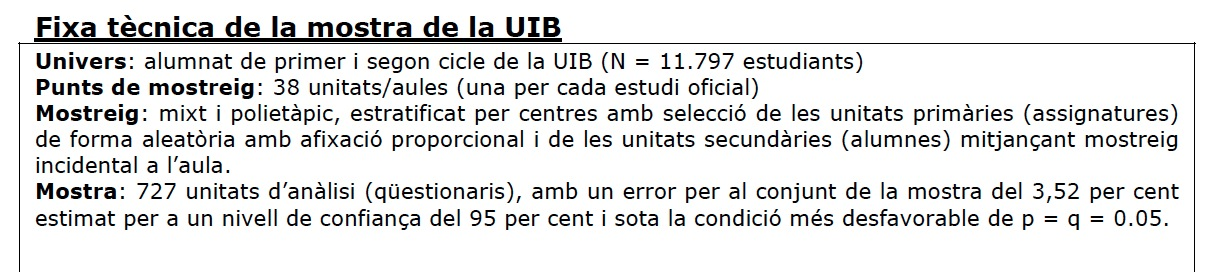
\includegraphics[width=1.1\linewidth]{plagiUIB2.jpg}
\end{center}
$$
\mbox{Error}= \hphantom{\frac{1.96}{\sqrt{727}}\approx 0.0363}
$$
\end{frame}



\begin{frame}
\frametitle{Exemple}
\blue{Volem estudiar quina fracció de les morts per càncer corresponen a morts per càncer d'estómac. Per determinar aquesta fracció a un nivell de confiança del 95\% i garantir un error màxim de 0.05, de quina mida ha de ser la mostra \emph{en el pitjor dels casos}?}


\end{frame}




\subsection{$\sigma$ de població normal}
\begin{frame}
\frametitle{Variància d'una població normal}


Considerem ara la situació següent:
\begin{itemize}
\item  $X$ una v.a. normal amb $\mu$ i $\sigma$ desconegudes

\item $X_1,\ldots,X_n$ una m.a.s. de $X$ i variància mostral $\widetilde{S}_X^2$
\end{itemize}


\begin{teorema}
En aquestes condicions
$$
\frac{(n-1) \tilde{S}_{X}^2}{\sigma^2}
$$
té distribució $\chi^2_{n-1}$
\end{teorema}
\end{frame}

\begin{frame}
\frametitle{Variància d'una població normal}


Considerem ara la situació següent:
\begin{itemize}
\item  $X$ una v.a. normal amb $\mu$ i $\sigma$ desconegudes

\item $X_1,\ldots,X_n$ una m.a.s. de $X$ i variància mostral $\widetilde{S}_X^2$
\end{itemize}


\begin{teorema}
En aquestes condicions,  un interval  de confiança del $(1-\alpha)\cdot 100\%$ per a \red{$\sigma^2$}
és  
$$
\left] \frac{(n-1)\widetilde{S}_{X}^2}{\chi_{n-1,1-\frac{\alpha}{2}}^2},
\frac{(n-1)\widetilde{S}_{X}^2}{\chi_{n-1,\frac{\alpha}{2}}^2}
\right[,
$$
on $\chi_{\nu,q}^2$ és el $q$-quantil de la distribució $\chi_{\nu}^2$
\end{teorema}
\end{frame}


\begin{frame}
\frametitle{Variància d'una població normal}

En efecte
$$
\begin{array}{l}
1-\alpha=P\left(\chi_{n-1,\frac{\alpha}{2}}^2\leq \chi_{n-1}^2\leq
\chi_{n-1,1-\frac{\alpha}{2}}^2\right)\\[2ex]
\quad\displaystyle =P\left(\chi_{n-1,\frac{\alpha}{2}}^2\leq \frac{(n-1) \widetilde{S}_{X}^2}{\sigma^2}\leq
\chi_{n-1,1-\frac{\alpha}{2}}^2
\right)\\[2ex]
\quad\displaystyle = P\left(\frac{(n-1)
\widetilde{S}_{X}^2}{\chi_{n-1,1-\frac{\alpha}{2}}^2}\leq\sigma^2\leq\frac{
(n-1)\widetilde{S}_{X}^2}{\chi_{n-1,\frac{\alpha}{2}}^2}
\right)
\end{array}
$$
I ara $\chi_{n-1}^2$ no és simètrica, així que s'han de calcular $\chi_{n-1,\frac{\alpha}{2}}^2$ i $\chi_{n-1,1-\frac{\alpha}{2}}^2$
\medskip

\blue{Observació:} L'interval de confiança per $\sigma^2$ no està
centrat en $\widetilde{S}_{X}^2$

\end{frame}


\begin{frame}
\frametitle{Exemple}

Un índex de qualitat d'un reactiu químic és el temps que triga a
actuar. L'estàndard és que aquest ha de ser $\leq 30$ segons.
Se suposa que la distribució del temps d'actuació del reactiu és
aproximadament normal. 
\medskip


Es realitzen 30 proves en les quals es mesura el temps
d'actuació del reactiu:
\medskip

12, 13, 13, 14, 14, 14, 15, 15, 16, 17, 17, 18, 18, 19, 19, 25, 25, 26, 27, 30,
33, 34, 35, 40, 40, 51, 51, 58, 59, 83
\medskip

Es demana calcular un interval de confiança per a la desviació típica al nivell
$95\%$
\end{frame}

\begin{frame}[fragile]
\frametitle{Exemple}
\red{$\displaystyle \left] \frac{(n-1)\widetilde{S}_{X}^2}{\chi_{n-1,1-\frac{\alpha}{2}}^2},
\frac{(n-1)\widetilde{S}_{X}^2}{\chi_{n-1,\frac{\alpha}{2}}^2}
\right[$}

\begin{verbatim}
> Temps=c(12,13,13,14,14,14,15,15,16,17,17,18,
 18,19,19,25,25,26,27,30,33,34,35,40,40,51,51,
 58,59,83)
> length(Temps) #n
[1]  30.0000
> var(Temps) # variància mostral
[1]  301.5506
\end{verbatim}
i  $\alpha=0.05$:
$$
\chi_{29,0.975}^2=45.72,\
\chi_{29,0.025}^2=16.05
$$
\end{frame}

\begin{frame} 
\frametitle{Exemple}

L'interval serà
$$
\left] \frac{(n-1)\widetilde{S}_{X}^2}{\chi_{n-1,1-\frac{\alpha}{2}}^2},
\frac{(n-1)\widetilde{S}_{X}^2}{\chi_{n-1,\frac{\alpha}{2}}^2}
\right[
$$
Obtenim
$$
\left] \frac{29\cdot 301.5506}{45.72},
\frac{29\cdot 301.5506}{16.05}
\right[=
\red{]191.27, 544.86[}
$$


Aquest era per a la variància! Per a la desviació típica
$$
]\sqrt{191.27}, \sqrt{544.86}[=\red{]13.83,23.34[}
$$

\end{frame}

\subsection{$N$ relativament petit}
\begin{frame}
\frametitle{``Poblacions finites''}
Fins ara hem emprat mostres aleatòries simples
\medskip

A la pràctica, sovint es prenen mostres aleatòries sense reposició
\medskip

Si la mida $N$ de la població és molt més gran que la mida $n$ de la mostra (posem $N\geq 40n$), les fórmules donades fins ara funcionen aproximadament bé
\medskip

Però\ldots
\vspace*{-4ex}

\begin{center}
\hspace*{-0.5cm}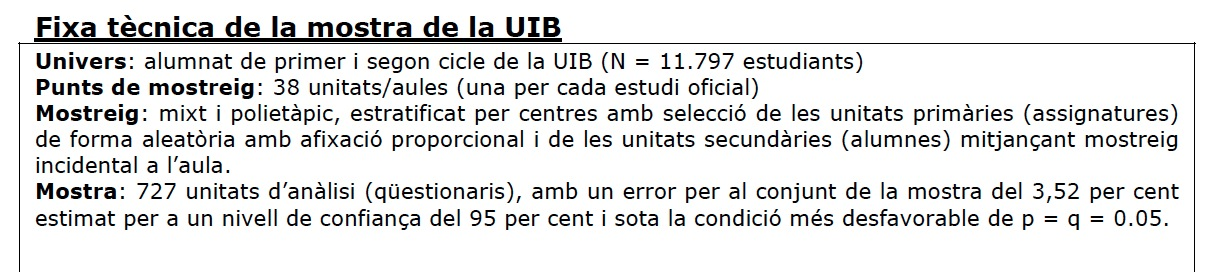
\includegraphics[width=1.1\linewidth]{plagiUIB2.jpg}
\end{center}


\end{frame}

\begin{frame}
\frametitle{``Poblacions finites''}

Es dóna l'efecte de \emph{població finita} quan $N$ és relativament petit
\medskip

En aquest cas, a les fórmules que hem donat per als intervals de confiança per a $\mu$ o $p$ cal multiplicar l'error estàndard o l'error mostral pel factor corrector
$$
\sqrt{\frac{N-n}{N-1}}
$$

\end{frame}

\begin{frame}
\frametitle{``Poblacions finites''}

Considerem  la situació següent:
\begin{itemize}
\item  $X$ una població de mida $N$ que segueix una distribució amb mitjana poblacional $\mu$ desconeguda

\item $X_1,\ldots,X_n$ una m.a.\ sense reposició de $X$, amb mitjana $\overline{X}$

\item  $n$ és gran 
\end{itemize}

\begin{block}{``Teorema''}
En aquestes condicions, es recomana prendre com a interval  de confiança del $(1-\alpha)\cdot 100\%$ per a $\mu$
$$
\left]\overline{X}-z_{1-\frac{\alpha}{2}}\frac{\sigma}{\sqrt{n}}\sqrt{\frac{N-n}{N-1}},\
    \overline{X}+z_{1-\frac{\alpha}{2}}\frac{\sigma}{\sqrt{n}}\sqrt{\frac{N-n}{N-1}}\right[
$$
\end{block}



\end{frame}




\begin{frame}
\frametitle{``Poblacions finites''}
\vspace*{-2ex}

Considerem  la situació següent:
\begin{itemize}
\item  $X$ una població de mida $N$ que segueix una distribució Bernoulli amb $p$ desconeguda

\item $X_1,\ldots,X_n$ una m.a.\ sense reposició de $X$, amb $n$ molt gran  i amb freqüència relativa d'èxits $\widehat{p}_{X}$ no extrema
\end{itemize}
\medskip

\begin{block}{``Teorema''}
En aquestes condicions, es recomana prendre com a interval  de confiança del $(1-\alpha)\cdot 100\%$ per a $p$
$$
\begin{array}{l}
\displaystyle \left]\widehat{p}_{X}-z_{1-\frac{\alpha}{2}}\sqrt{\frac{\widehat{p}_{X}
(1-\widehat{p}_{X})}{n}}\sqrt{\frac{N-n}{N-1}}\right.,\\[1ex]
\hspace*{3cm}\displaystyle
\left.\widehat{p}_{X}+z_{1-\frac{\alpha}{2}}\sqrt{\frac{\widehat{p}_{X}
(1-\widehat{p}_{X})}{n}}\sqrt{\frac{N-n}{N-1}}\right[
\end{array}$$
\end{block}
\end{frame}


\begin{frame}
\frametitle{``Poblacions finites''}

\begin{block}{``Teorema''}
En les condicions anteriors, per obtenir un interval de confiança del $(1-\alpha)\cdot 100\%$ per a $p$ en el pitjor dels casos caldrà prendre una mostra de mida
$$
n=\left\lceil\frac{Nz_{1-\frac{\alpha}{2}}^2}{A^2(N-1)+z_{1-\frac{\alpha}{2}}^2}\right\rceil
$$
\end{block}
\end{frame}

\begin{frame}
\frametitle{Exemple}
\vspace*{-5ex}

\begin{center}
\hspace*{-0.5cm}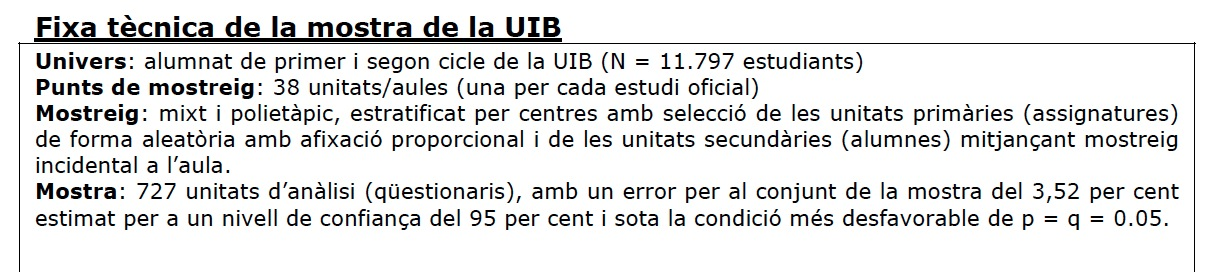
\includegraphics[width=1.1\linewidth]{plagiUIB2.jpg}
\end{center}

\blue{De la població total d'estudiants de grau de la UIB quants d'hem d'escollir de manera aleatòria sense reposició per estimar la proporció dels que han comès plagi, amb un error del 3.52\% i un nivell de confiança del 95\%?}
\end{frame}




\end{document}

